\section{Casi d'uso} \label{casi uso}

    In questa sezione vengono riportati i casi d'uso rilevati dal team dopo un'attenta analisi dei requisiti e
    vari incontri con la \glossaryItem{Proponente}.
    Nel descrivere ogni caso d'uso si utilizza una struttura contenente le seguenti voci:

        \begin{itemize}

            \item \textbf{ID} - Codice identificativo e univoco la cui formattazione è specificata all'interno del
            documento \vNormeDiProgetto;
            \item \textbf{Nome} - Titolo del caso d'uso;
            \item \textbf{Attori} - Elenco degli \glossaryItem{attori} principali e secondari del caso d'uso in questione;
            \item \textbf{Descrizione} - Breve descrizione del caso d'uso;
            \item \textbf{Precondizione} - Condizione che deve essere vera prima dell'esecuzione delle azioni contenute nel caso d'uso;
            \item \textbf{Postcondizione} - Condizione che deve essere vera dopo l'esecuzione delle azioni contenute nel
            caso d'uso;
            \item \textbf{Scenario principale} - Rappresenta il flusso degli eventi;
            \item \textbf{Inclusioni} - Utilizzate per evitare di descrivere più volte lo stesso flusso di eventi;
            \item \textbf{Estensioni} - Modellano la parte opzionale di un caso d'uso.

        \end{itemize}

    Per alcuni casi d'uso vengono utilizzati gli \glossaryItem{Use Case Diagram} per rendere la descrizione più
    semplice e fruibile.

    \subsection{Attori} \label{attori}

        Il nostro applicativo è suddiviso in 2 moduli:

        \begin{itemize}

            \item Il primo modulo si occupa della configurazione e dell'avvio di una procedura \glossaryItem{Batch} che accederà successivamente
            alle funzionalità del secondo modulo periodicamente. In questo scenario l'attore principale è un utente umano
            che configura la procedura e successivamente la avvia;
            \item Il secondo modulo si occupa invece della raccolta dei dati (traces nel nostro caso) utili a monitorare l'eventuale
            scatenarsi di critical event. In questo scenario l'attore principale è la Procedura Batch in quanto accede al
            modulo come entità esterna e ne utilizza le funzionalità.

        \end{itemize}

        Dai due moduli sono quindi emersi i seguenti attori:

        \begin{itemize}

            \item \textbf{Amministratore di sistema}

                L'amministratore di sistema è un utente umano che ha accesso al server \glossaryItem{ElasticSearch} e può modificare i
                parametri di avvio della procedura automatica;

            \item \textbf{Procedura Batch}

                Una procedura automatica che, una volta avviata, accede alle funzionalità offerte dal sistema come il calcolo
                delle metriche o l'aggiornamento delle baseline.

        \end{itemize}

        Infine, merita un'analisi anche \textbf{ElasticSearch}. All'interno della nostra applicazione ElasticSearch viene utilizzato
        in due modi:

        \begin{itemize}

            \item Server dove vengono salvate e mantenute tutte le configurazioni necessarie al corretto funzionamento del
            sistema. Le configurazioni sono modificabili dal sistema;
            \item Server da cui recuperare i dati (traces) per le elaborazioni. I dati non possono essere modificati dal
            sistema.

        \end{itemize}

        ElasticSearch è quindi un attore del nostro sistema, ma solo nel secondo caso, cioè nella raccolta di traces.

\newpage

    \subsection{Descrizione casi d'uso} \label{descr casi uso}

        In questa sezione verranno elencati i casi d'uso. \\
        L'ordine è rilevante in quanto, UC1 e UC2 descrivono le funzionalità del primo modulo dell'applicazione e
        i restanti descrivono le funzionalità del secondo modulo. \\
        L'attore procedura Batch è interno al sistema nel primo modulo e diventa esterno nel secondo.

        \subsubsection{UC1 - Configurazione schedulazione procedura Batch}

            \begin{figure}[H]
                \centering
                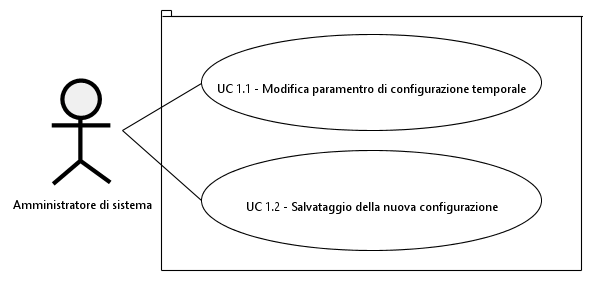
\includegraphics[width=13cm,height=13cm,keepaspectratio]{./images/UC1.png}
                \caption{UC1 - Configurazione schedulazione della procedura Batch}
            \end{figure}

            \begin{itemize}

                \item \textbf{Attori} - Amministratore di sistema;
                \item \textbf{Descrizione} - L'attore configura la schedulazione temporale della procedura Batch, cioè la
                sua periodicità di esecuzione;
                \item \textbf{Precondizione} - L'attore ha accesso al sistema;
                \item \textbf{Postcondizione} - L'attore ha configurato la schedulazione della procedura Batch;
                \item \textbf{Scenario principale}

                    \begin{enumerate}

                        \item L'attore modifica il parametro di configurazione temporale (UC1.1);
                        \item L'attore salva la nuova configurazione della schedulazione (UC1.2).

                    \end{enumerate}

            \end{itemize}

            \subsubsection{UC1.1 - Modifica parametro di configurazione temporale}

                \begin{itemize}

                    \item \textbf{Attori} - Amministratore di sistema;
                    \item \textbf{Descrizione} - L'attore modifica il parametro di configurazione della schedulazione per la
                    procedura Batch;
                    \item \textbf{Precondizione} - L'attore ha accesso al sistema;
                    \item \textbf{Postcondizione} - L'attore ha modificato i parametri di configurazione;
                    \item \textbf{Scenario principale} - L'attore modifica i parametri di configurazione.

                \end{itemize}

            \subsubsection{UC1.2 - Salvataggio della nuova configurazione}

                \begin{itemize}

                    \item \textbf{Attori} - Amministratore di sistema;
                    \item \textbf{Descrizione} - L'attore salva la nuova configurazione della schedulazione della procedura Batch;
                    \item \textbf{Precondizione} - L'attore ha modificato i parametri di configurazione;
                    \item \textbf{Postcondizione} - L'attore ha salvato i parametri di configurazione;
                    \item \textbf{Scenario principale} - L'attore salva la nuova configurazione della schedulazione della procedura Batch.

                \end{itemize}

\newpage

        \subsubsection{UC2 - Avvio esecuzione procedura Batch}

			\begin{figure}[H]
                \centering
                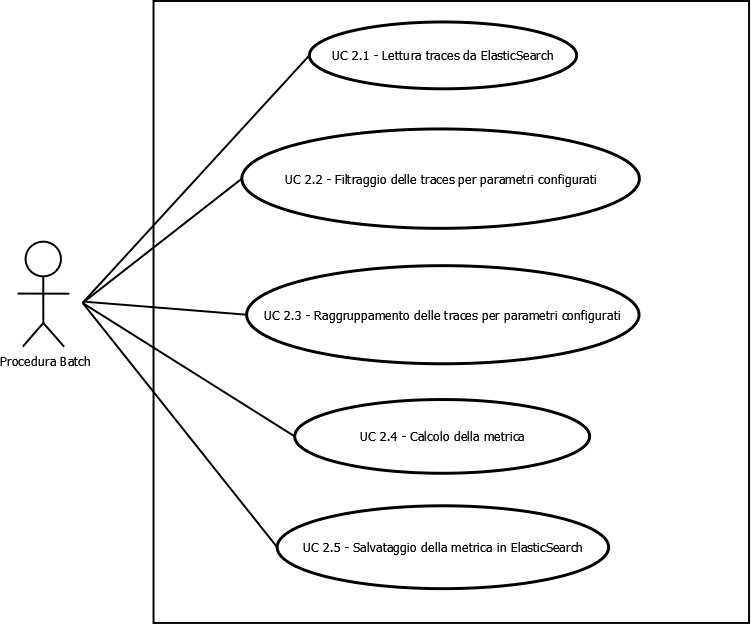
\includegraphics[width=13cm,height=13cm,keepaspectratio]{./images/UC2.png}
                \caption{UC2 - Avvio esecuzione procedura Batch}
            \end{figure}

            \begin{itemize}

                \item \textbf{Attori} - Amministratore di sistema;
                \item \textbf{Descrizione} - L'attore avvia l'esecuzione della procedura Batch;
                \item \textbf{Precondizione} - L'attore ha accesso al sistema;
                \item \textbf{Postcondizione} - L'attore ha avviato l'esecuzione della procedura Batch;
                \item \textbf{Scenario principale} - L'attore avvia l'esecuzione della procedura Batch.

            \end{itemize}

\newpage

        \subsubsection{UC3 - Generazione metrica}

            \begin{figure}[H]
                \centering
                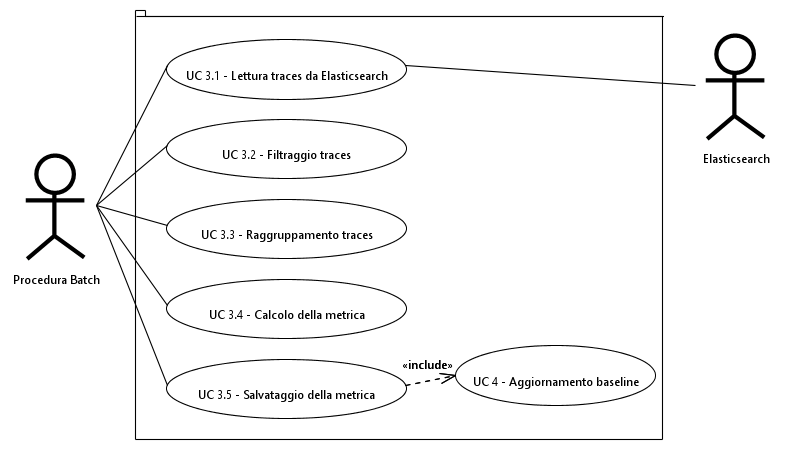
\includegraphics[width=13cm,height=17cm,keepaspectratio]{./images/UC3.png}
                \caption{UC3 - Generazione metrica}
            \end{figure}

            \begin{itemize}

                \item \textbf{Attori} - Procedura Batch, ElasticSearch;
                \item \textbf{Descrizione} - La procedura Batch legge traces da ElasticSearch, le filtra, le raggruppa,
                calcola la metrica a partire dalle traces e salva il risultato;
                \item \textbf{Precondizione} - La procedura Batch è stata avviata;
                \item \textbf{Postcondizione} - La metrica è stata calcolata e salvata;
                \item \textbf{Scenario principale}

                    \begin{enumerate}

                        \item La procedura Batch legge le traces da indice di ElasticSearch (UC3.1);
                        \item La procedura Batch filtra le traces (UC3.2);
                        \item La procedura Batch raggruppa le traces (UC3.3);
                        \item La procedura Batch calcola la metrica (UC3.4);
                        \item La procedura Batch salva la metrica (UC3.5).

                    \end{enumerate}

            \end{itemize}

                \subsubsection{UC3.1 - Lettura traces da ElasticSearch}

                    \begin{itemize}

                        \item \textbf{Attori} - Procedura Batch, ElasticSearch;
                        \item \textbf{Descrizione} - La procedura Batch legge le traces da un indice ElasticSearch;
                        \item \textbf{Precondizione} - La procedura Batch è stata avviata;
                        \item \textbf{Postcondizione} - Le traces sono state lette da indice ElasticSearch;
                        \item \textbf{Scenario principale} - La procedura Batch legge le traces da un indice ElasticSearch.

                    \end{itemize}
                
                \subsubsection{UC3.2 - Filtraggio traces}

                    %\begin{figure}[H]
                    %    \centering
                    %    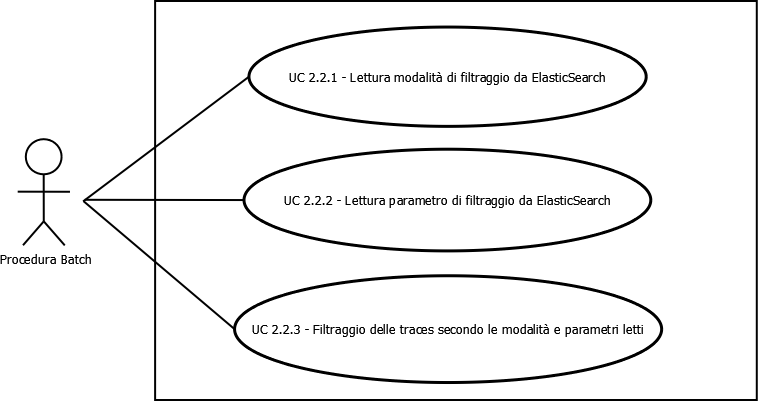
\includegraphics[width=13cm,height=13cm,keepaspectratio]{./images/UC2_2.png}
                    %    \caption{UC2.2 - filtraggio delle traces per parametri configurati}
                    %\end{figure}

                    \begin{itemize}

                        \item \textbf{Attori} - Procedura Batch;
                        \item \textbf{Descrizione} - L'attore filtra le traces per eliminare quelle non utili al calcolo;
                        \item \textbf{Precondizione} - L'attore ha letto le traces coinvolte nel calcolo da indice ElasticSearch;
                        \item \textbf{Postcondizione} - Le traces sono state filtrate;
                        \item \textbf{Scenario principale} - L'attore filtra le traces.

                    \end{itemize}

                \subsubsection{UC3.3 - Raggruppamento traces}

                    %\begin{figure}[H]
                    %    \centering
                    %    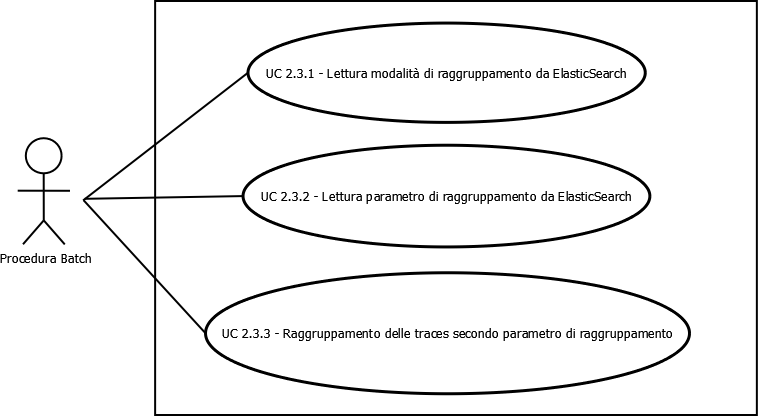
\includegraphics[width=13cm,height=13cm,keepaspectratio]{./images/UC2_3.png}
                    %    \caption{UC2.3 - Raggruppamento delle traces per parametri configurati}
                    %\end{figure}

                    \begin{itemize}

                        \item \textbf{Attori} - Procedura Batch;
                        \item \textbf{Descrizione} - L'attore raggruppa le traces per suddividerle in sottoinsiemi;
                        \item \textbf{Precondizione} - L'attore ha filtrato le traces coinvolte nel calcolo;
                        \item \textbf{Postcondizione} - Le traces sono state raggruppate;
                        \item \textbf{Scenario principale} - L'attore raggruppa le traces.

                    \end{itemize}

                \subsubsection{UC3.4 - Calcolo della metrica}

                    %\begin{figure}[H]
                    %    \centering
                    %    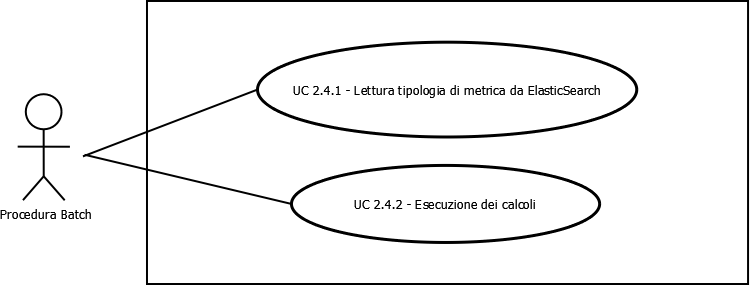
\includegraphics[width=13cm,height=10cm,keepaspectratio]{./images/UC2_4.png}
                    %    \caption{UC2.4 - Calcolo della metrica}
                    %\end{figure}

                    \begin{itemize}

                        \item \textbf{Attori} - Procedura Batch;
                        \item \textbf{Descrizione} - L'attore esegue i calcoli per produrre la metrica;
                        \item \textbf{Precondizione} - L'attore ha raggruppato le traces;
                        \item \textbf{Postcondizione} - L'attore ha calcolato la metrica;
                        \item \textbf{Scenario principale} - L'attore calcola la metrica.

                    \end{itemize}

                \subsubsection{UC3.5 - Salvataggio della metrica}

                    \begin{itemize}

                        \item \textbf{Attori} - Procedura Batch;
                        \item \textbf{Descrizione} - L'attore salva la metrica precedentemente calcolata;
                        \item \textbf{Precondizione} - L'attore ha calcolato la metrica;
                        \item \textbf{Postcondizione} - L'attore ha salvato la metrica;
                        \item \textbf{Scenario principale} - L'attore salva la metrica;
                        \item \textbf{Inclusione} - Ad ogni salvataggio di una metrica, automaticamente viene eseguito UC4,
                        cioè viene aggiornata la baseline costruita per tale metrica.

                    \end{itemize}

\newpage

            \subsubsection{UC4 - Aggiornamento baseline}

                \begin{figure}[H]
                    \centering
                    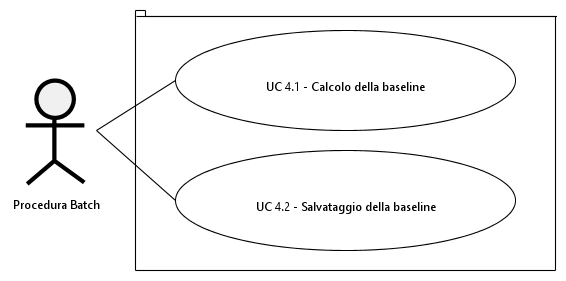
\includegraphics[width=13cm,height=15cm,keepaspectratio]{./images/UC4.png}
                    \caption{UC4 - Aggiornamento baseline}
                \end{figure}

                \begin{itemize}

                    \item \textbf{Attori} - Procedura batch;
                    \item \textbf{Descrizione} - L'attore crea una baseline o aggiorna una baseline già esistente all'inserimento
                    di una metrica e, successivamente, la salva;
                    \item \textbf{Precondizione} - Una metrica è stata salvata (UC3.5);
                    \item \textbf{Postcondizione} - La baseline è stata salvata;
                    \item \textbf{Scenario principale}

                        \begin{enumerate}

                            \item L'attore calcola la baseline (UC4.1);
                            \item L'attore salva la baseline (UC4.2).

                        \end{enumerate}

                \end{itemize}

                \subsubsection{UC4.1 - Calcolo della baseline}

                    \begin{itemize}

                        \item \textbf{Attori} - Procedura batch;
                        \item \textbf{Descrizione} - L'attore calcola la baseline o ne aggiorna una esistente a partire dalla
                        metrica appena salvata;
                        \item \textbf{Precondizione} - Una metrica è stata salvata (UC3.5);
                        \item \textbf{Postcondizione} - L'attore ha calcolato la baseline;
                        \item \textbf{Scenario principale} - L'attore calcola la baseline.

                    \end{itemize}

                \subsubsection{UC4.2 - Salvataggio della baseline}

                    \begin{itemize}

                        \item \textbf{Attori} - Procedura batch;
                        \item \textbf{Descrizione} - L'attore salva la baseline precedentemente calcolata per poterla
                        successivamente utilizzare;
                        \item \textbf{Precondizione} - L'attore ha calcolato la baseline;
                        \item \textbf{Postcondizione} - L'attore ha salvato la baseline;
                        \item \textbf{Scenario principale} - L'attore salva la baseline.

                \end{itemize}

\newpage

            \subsubsection{UC5 - Controllo critical event}

                \begin{figure}[H]
                    \centering
                    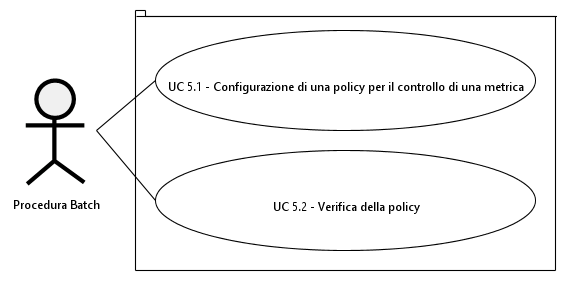
\includegraphics[width=13cm,height=13cm,keepaspectratio]{./images/UC5.png}
                    \caption{UC5 - Controllo di critical event}
                \end{figure}

                \begin{itemize}

                    \item \textbf{Attori} - Procedura batch;
                    \item \textbf{Descrizione} - All'aggiunta di una metrica, l'attore configura una policy
                    per quel tipo di metrica, controlla se è stata violata e lancia un'azione di rimedio se l'esito è positivo;
                    \item \textbf{Precondizione} - Una metrica è stata salvata ed è stata calcolata o aggiornata la relativa
                    baseline;
                    \item \textbf{Postcondizione} - L'attore notifica se è stata violata una policy;
                    \item \textbf{Scenario principale}
                        \begin{enumerate}

                            \item L'attore configura la policy per il controllo della metrica (UC5.1);
                            \item L'attore verifica se i valori della metrica superano le soglie della policy (UC5.2).

                        \end{enumerate}

                \end{itemize}

                \subsubsection{UC5.1 - Configurazione della policy per il controllo della metrica}

                    %\begin{figure}[H]
                    %    \centering
                    %    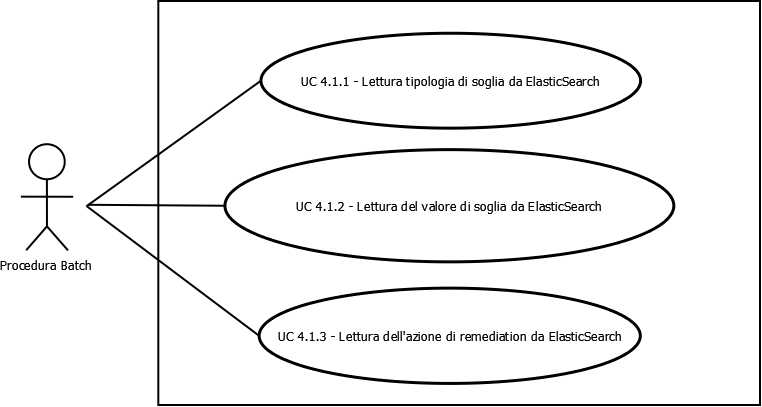
\includegraphics[width=13cm,height=13cm,keepaspectratio]{./images/UC4_1.png}
                    %    \caption{UC4.1 - Configurazione della policy per il controllo della metrica da ElasticSearch}
                    %\end{figure}

                    \begin{itemize}

                        \item \textbf{Attori} - Procedura batch;
                        \item \textbf{Descrizione} - L'attore configura una policy da utilizzare per il controllo della
                        metrica;
                        \item \textbf{Precondizione} - Una metrica è stata salvata ed è stata calcolata o aggiornata la relativa
                        baseline;
                        \item \textbf{Postcondizione} - L'attore ha configurato una policy di controllo sulla metrica;
                        \item \textbf{Scenario principale} - L'attore configura una policy.

                    \end{itemize}

                \subsubsection{UC5.2 - Verifica della policy}

                    \begin{itemize}

                        \item \textbf{Attori} - Procedura batch;
                        \item \textbf{Descrizione} - L'attore verifica se la metrica supera le soglie della policy e agisce di
                        conseguenza;
                        \item \textbf{Precondizione} - L'attore ha configurato la policy per il controllo della metrica;
                        \item \textbf{Postcondizione} - L'attore ha verificato se la metrica ha superato le soglie della policy;
                        \item \textbf{Scenario principale} - L'attore verifica la policy e lancia un'azione di rimedio in caso di violazione
                        della stessa.

                    \end{itemize}

\newpage

            \subsubsection{UC6 - Invio messaggio di posta elettronica}

                \begin{figure}[H]
                    \centering
                    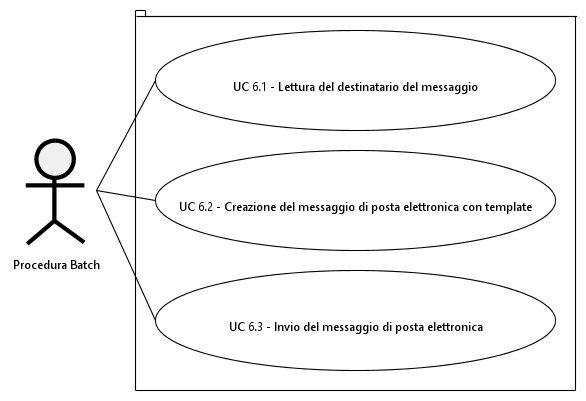
\includegraphics[width=13cm,height=13cm,keepaspectratio]{./images/UC6.png}
                    \caption{UC6 - Invio messaggio di posta elettronica}
                \end{figure}

                \begin{itemize}

                    \item \textbf{Attori} - Procedura batch;
                    \item \textbf{Descrizione} - L'attore invia una e-mail di notifica se il risultato di UC5 è positivo;
                    \item \textbf{Precondizione} - UC5 ha dato esito positivo e l'azione da compiere è l'invio di una e-mail di notifica;
                    \item \textbf{Postcondizione} - L'attore ha inviato una e-mail di notifica;
                    \item \textbf{Scenario principale}
                        \begin{enumerate}

                            \item L'attore legge il destinatario del messaggio (UC6.1);
                            \item L'attore crea la e-mail a partire da un template (UC6.2);
                            \item L'attore invia il messaggio di notifica (UC6.3).

                        \end{enumerate}

                \end{itemize}

                \subsubsection{UC6.1 - Lettura del destinatario del messaggio}

                    \begin{itemize}

                        \item \textbf{Attori} - Procedura batch;
                        \item \textbf{Descrizione} - L'attore legge il destinatario del messaggio di posta elettronica;
                        \item \textbf{Precondizione} - UC5 ha dato esito positivo e l'azione da compiere è l'invio di una e-mail di notifica;
                        \item \textbf{Postcondizione} - L'attore ha letto il destinatario della e-mail;
                        \item \textbf{Scenario principale} - L'attore legge il destinatario della e-mail.

                    \end{itemize}

                \subsubsection{UC6.2 - Creazione messaggio di posta elettronica con template}

                    \begin{itemize}

                        \item \textbf{Attori} - Procedura batch;
                        \item \textbf{Descrizione} - L'attore crea il messaggio di notifica del critical event utilizzando un
                        template e il destinatatio precedentemente letto;
                        \item \textbf{Precondizione} - L'attore ha letto il destinatario del messaggio;
                        \item \textbf{Postcondizione} - L'attore ha creato il messaggio;
                        \item \textbf{Scenario principale} - L'attore crea il messaggio.

                    \end{itemize}

                \subsubsection{UC6.3 - Invio del messaggio di posta elettronica}

                    \begin{figure}[H]
                        \centering
                        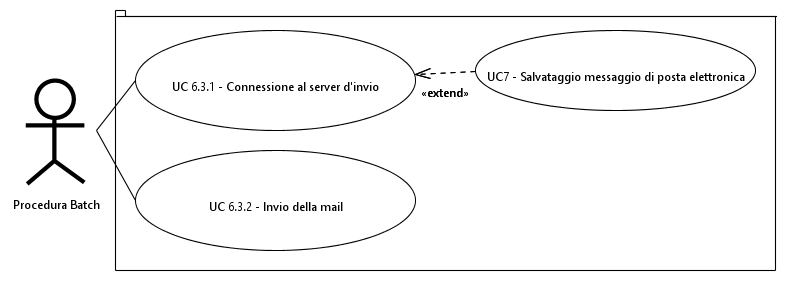
\includegraphics[width=13cm,height=13cm,keepaspectratio]{./images/UC6_3.png}
                        \caption{UC6.3 - Invio del messaggio di posta elettronica}
                    \end{figure}

                    \begin{itemize}

                        \item \textbf{Attori} - Procedura batch;
                        \item \textbf{Descrizione} - L'attore invia il messaggio creato dopo essersi connesso al server;
                        \item \textbf{Precondizione} - L'attore ha creato il messaggio da inviare;
                        \item \textbf{Postcondizione} - L'attore ha inviato il messaggio;
                        \item \textbf{Scenario principale}
                            \begin{enumerate}

                                \item L'attore si connette al server per l'invio della mail (UC6.3.1);
                                \item L'attore invia la mail (UC6.3.2).

                            \end{enumerate}

                    \end{itemize}

                    \subsubsection{UC6.3.1 - Connessione al server di invio}

                        \begin{itemize}

                            \item \textbf{Attori} - Procedura batch;
                            \item \textbf{Descrizione} - L'attore si connette al server di invio della mail;
                            \item \textbf{Precondizione} - L'attore ha creato il messaggio da inviare;
                            \item \textbf{Postcondizione} - L'attore si è connesso al server;
                            \item \textbf{Scenario principale} - L'attore si connette al server di invio delle mail;
                            \item \textbf{Estensione} - Nel caso in cui l'attore non riesca a connettersi al server, il messaggio viene 									memorizzato per un invio futuro (UC7).

                        \end{itemize}

                    \subsubsection{UC6.3.2 - Invio della mail}

                        \begin{itemize}

                            \item \textbf{Attori} - Procedura batch;
                            \item \textbf{Descrizione} - L'attore dopo essersi collegato al server di invio, spedisce il
                            messaggio di posta elettronica;
                            \item \textbf{Precondizione} - L'attore si è connesso al server di invio;
                            \item \textbf{Postcondizione} - L'attore ha inviato la mail;
                            \item \textbf{Scenario principale} - L'attore invia la mail.

                        \end{itemize}

\newpage

            \subsubsection{UC7 - Salvataggio messaggio di posta elettronica}

				\begin{figure}[H]
    	            \centering
        	        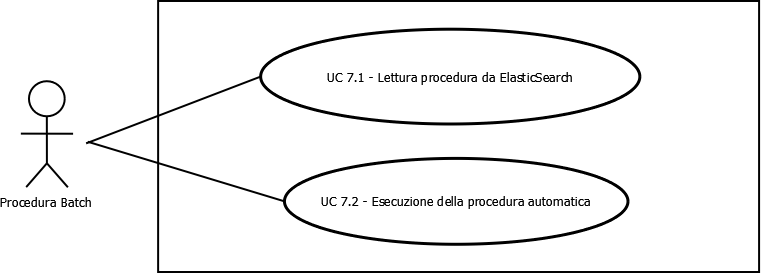
\includegraphics[width=13cm,height=13cm,keepaspectratio]{./images/UC7.png}
            	    \caption{UC7 - Salvataggio messaggio di posta elettronica}
            	\end{figure}

                \begin{itemize}

                    \item \textbf{Attori} - Procedura batch;
                    \item \textbf{Descrizione} - L'attore salva il messaggio di posta elettronica non inviato a causa
                    di un errore di connessione al server di invio;
                    \item \textbf{Precondizione} - L'attore ha fallito la connessione al server;
                    \item \textbf{Postcondizione} - L'attore ha salvato il messaggio;
                    \item \textbf{Scenario principale} - L'attore salva la e-mail.

                \end{itemize}

\newpage

            \subsubsection{UC8 - Salvataggio critical event}

                \begin{figure}[H]
                    \centering
                    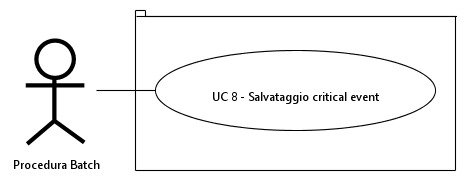
\includegraphics[width=13cm,height=10cm,keepaspectratio]{./images/UC8.png}
                    \caption{UC8 - Salvataggio critical event}
                \end{figure}

                \begin{itemize}

                    \item \textbf{Attori} - Procedura batch;
                    \item \textbf{Descrizione} - L'attore, successivamente allo scatenarsi di un critical event, salva le informazioni
                    dell'evento;
                    \item \textbf{Precondizione} - UC5 ha dato esito positivo;
                    \item \textbf{Postcondizione} - L'attore ha salvato le informazioni del critical event;
                    \item \textbf{Scenario principale} - L'attore salva le informazioni del critical event.

                \end{itemize}

\newpage

            \subsubsection{UC9 - Esecuzione procedura automatica}

                \begin{figure}[H]
                    \centering
                    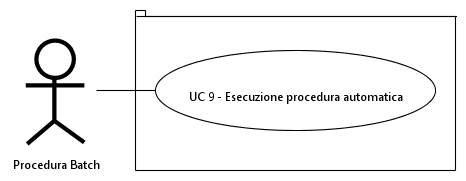
\includegraphics[width=13cm,height=10cm,keepaspectratio]{./images/UC9.png}
                    \caption{UC9 - Esecuzione procedura automatica}
                \end{figure}

                \begin{itemize}

                    \item \textbf{Attori} - Procedura batch;
                    \item \textbf{Descrizione} - L'attore esegue una procedura automatica a seguito di un critical event ricevuto;
                    \item \textbf{Precondizione} - UC5 ha dato esito positivo e richiede l'avvio di una procedura automatica;
                    \item \textbf{Postcondizione} - L'attore ha eseguito la procedura;
                    \item \textbf{Scenario principale} - L'attore esegue una procedura automatica.

                \end{itemize}

	    
                
            
		